\documentclass{article}

\usepackage{amsmath}
\usepackage{amssymb}
\usepackage{float}
\usepackage{graphicx}
\usepackage{tikz}
\usepackage{textpos}
\usepackage{minitoc} %% Required
\usepackage{pdfpages}

\usepackage[colorlinks=true, allcolors=blue]{hyperref}

\title{Lista 3}
\author{Luís Felipe Ramos Ferreira}
\date{\href{mailto:lframos.lf@gmail.com}{\texttt{lframos.lf@gmail.com}}
}

\begin{document}

\maketitle

\begin{itemize}
	\item (5.8.1) Exercício feito à mão e página com ele está anexado ao fim do pdf.

	\item (5.8.2)

	      Queremos provar o teorema de Turán, que diz que se um grafo \(G\) com \(n\) vértices é livre de \(K_r\), então:

	      \[|E(G)| \leq (1 - \frac{1}{r-1})\frac{n^2}{2}\]

	      Sabemos, a partir do teorema 5.3.11 do livro (que devemos usar na prova), que todo grafo \(G\) possui em sua estrutura uma clique de tamanho pelo menos \(\sum_{v \in V(G)} \frac{1}{n - d(v)}\),
	      onde \(d(v)\) é o grau de \(v\) em \(G\). Isso pois todo conjunto independente em \(G\) é uma clique em \(\overline{G}\).

	      Vamos inicialmente então assumir que o grafo \(G\) é livre de \(K_r\), a clique com \(r\) vértices. Disso podemos assumir que:

	      \[\sum_{v \in V(G)} \frac{1}{n - d(v)} \leq r -1\]

	      Como \(\frac{1}{n - d(v)}\) é uma função convexa em relação a \(d(v)\), podemos aplicar a transformação:

	      \[\frac{n}{n - \sum_{v \in V(G)} \frac{d(v)}{n}} \leq r - 1\]
	      \[\frac{n}{n - \frac{2 |E(G)|}{n}} \leq r - 1\]
	      \[\frac{n}{r - 1} \leq n - \frac{2 |E(G)|}{n}\]
	      \[\frac{2 |E(G)|}{n} \leq n - \frac{n}{r - 1}\]
	      \[\frac{2 |E(G)|}{n} \leq n (1 - \frac{1}{r - 1})\]
	      \[|E(G)| \leq \frac{n^2}{2} (1 - \frac{1}{r - 1})\]

	      Como queríamos demonstrar.


	\item (5.8.3)

	      Para resolver essa questão também usaremos o teorema 5.3.11 do livro. Seja \(G\) um grafo com \(n\) vértices e \(\pi = [v_1, \dots, v_{n}]\) uma permutação
	      aleatória e uniforme dos vértices de \(G\). Denotamos por \(\mathcal{N}(v)\) a vizinhança aberta de \(v\) em \(G\).

	      Vamos construir um conjunto \(S\) da seguinte maneira gulosa. Primeiro, escolha o vértice \(v\) de menor grau em \(G\) e adicione ele em \(S\).
	      Depois, remova de \(G\) tanto o próprio \(v\) como também a vizinhança de \(v\), \(\mathcal{N}(v)\). Continuamos o processo até \(V(G) = \emptyset\).

	      Trivialmente, \(S\) é um conjunto independente.






	\item (5.8.4)

	      Vamos utilizar \(\mu = \mathbb{E}[X]\) pois a notação é melhor. Queremos provar então que:

	      \[\mathbb{P}(X \geq \mathbb{E}[X] + t \sigma) \leq \frac{1}{1 + t^2}\]

	      Seja \(Z = X - \mathbb{E}[X]\). Sabemos que \(\mathbb{E}[Z] = 0\) e \(Var[Z] = \mathbb{E}[Z^2] = \sigma^2\)
	      e seja \(u = \frac{\sigma}{t}\). Então:

	      \(\mathbb{P}(X \geq \mathbb{E}[X] + t \sigma) = \mathbb{P}(Z \geq t \sigma) \leq \mathbb{P}((Z + u)^2 \geq (t \sigma + u)^2)\)

	      Pela Desigualdade de Markov, sabemos que:

	      \[\mathbb{P}((Z + u)^2 \geq (t \sigma + u)^2) \leq \frac{\mathbb{E}[(Z + u)^2]}{(t \sigma+ u)^2} = \frac{\mathbb{E}(Z^2) + 2u\mathbb{E}[Z] + u^2}{(t\sigma + u)^2} = \frac{\sigma^2 + u^2}{(t \sigma + u)^2}\]

	      O resto das contas foi feito a mão:

	      \begin{figure}[H]
		      \centering
		      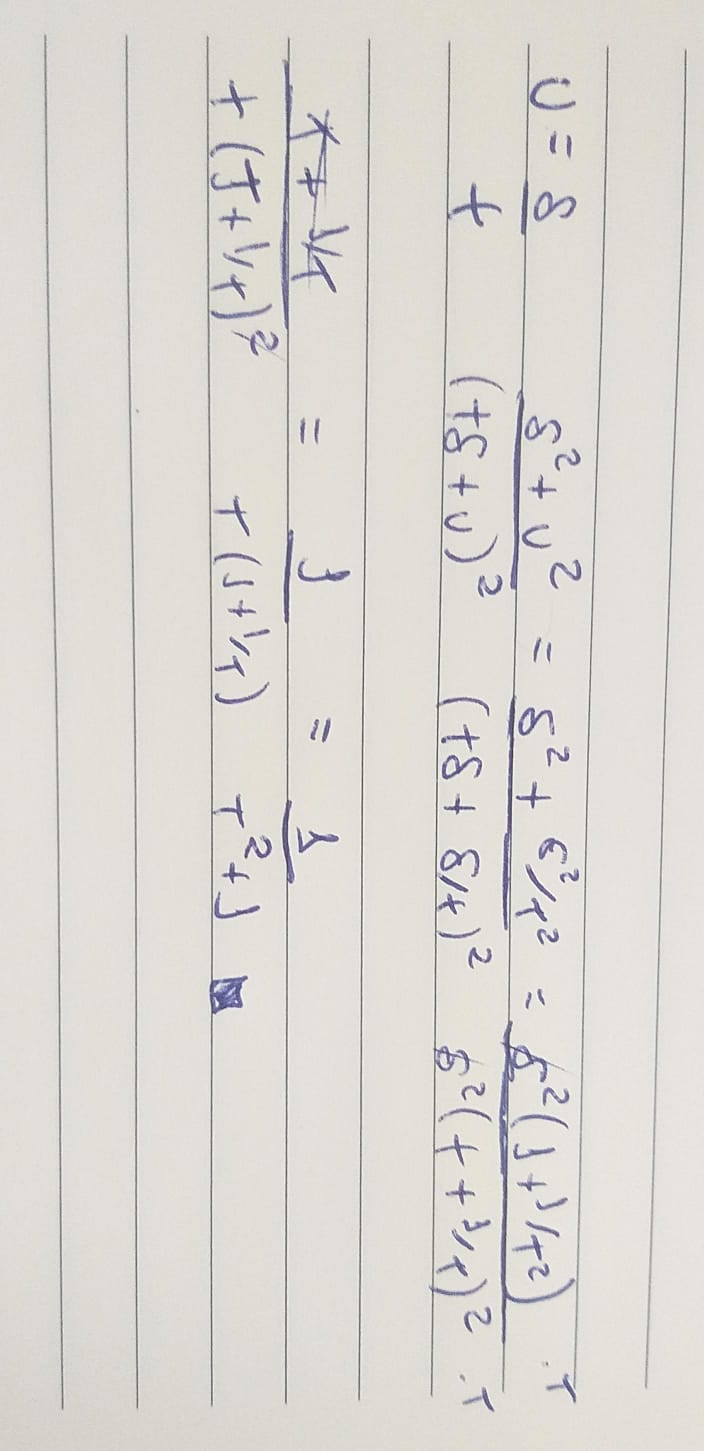
\includegraphics[angle=90,origin=c,width=0.8\textwidth]{images/584.jpeg}
	      \end{figure}

	      Portanto, provamos a desigualdade de Chantelli.


	\item (5.8.5)
	\item (5.8.6)

	      Queremos mostrar que \(R(4, k) \geq (\frac{ck}{log k})^2\) para \(k\) suficientemente grande.

	      Seja \(n = (\frac{k}{4 log k})^2\). Mostraremos que existe um grafo \(G\) com \(\frac{n}{2}\) vértices que é livre de \(K_4\) e satisfaz \(\alpha(G) < k\).
	      Consideremos o grafo \(G(n,p)\) com \(p = n^{-\frac{3}{4}}\). Pelo teorema 5.4.2, temos com alta probabilidade:

	      \[\alpha(G) \leq \frac{2 log n}{p} < k\]

	      Uma vez que \(n < k^2\) e, portanto, \(log n < 2 log k\).

	      Seja \(X\) a variável aleatória que representa o número de \(K_4\) em \(G(n, p)\). Temos que:

	      \[\mathbb{E}[X] = p^4 \binom{n}{4} \leq \frac{p^4 n^4}{24} = \frac{n^{-\frac{-3}{4} 4} n ^ 4}{24} = \frac{n}{24}\]

	      Pela desigualdade de markov, temos:

	      \[\mathbb{P}(X \geq \frac{n}{2}) \leq \frac{2}{n}\mathbb{E}[X]  = \frac{2}{n} \frac{n}{24} \leq \frac{1}{12}\]

	      Segue que existe um grafo \(H\) com \(n\) vértices, \(\alpha(H) < k\), que contém no
	      máximo \(n/2\) triângulos. Removendo no máximo \(n/2\) vértices de \(H\) (um para
	      cada triângulo), obtemos um grafo \(G\) como desejado inicialmente.

	\item (5.8.7)
\end{itemize}
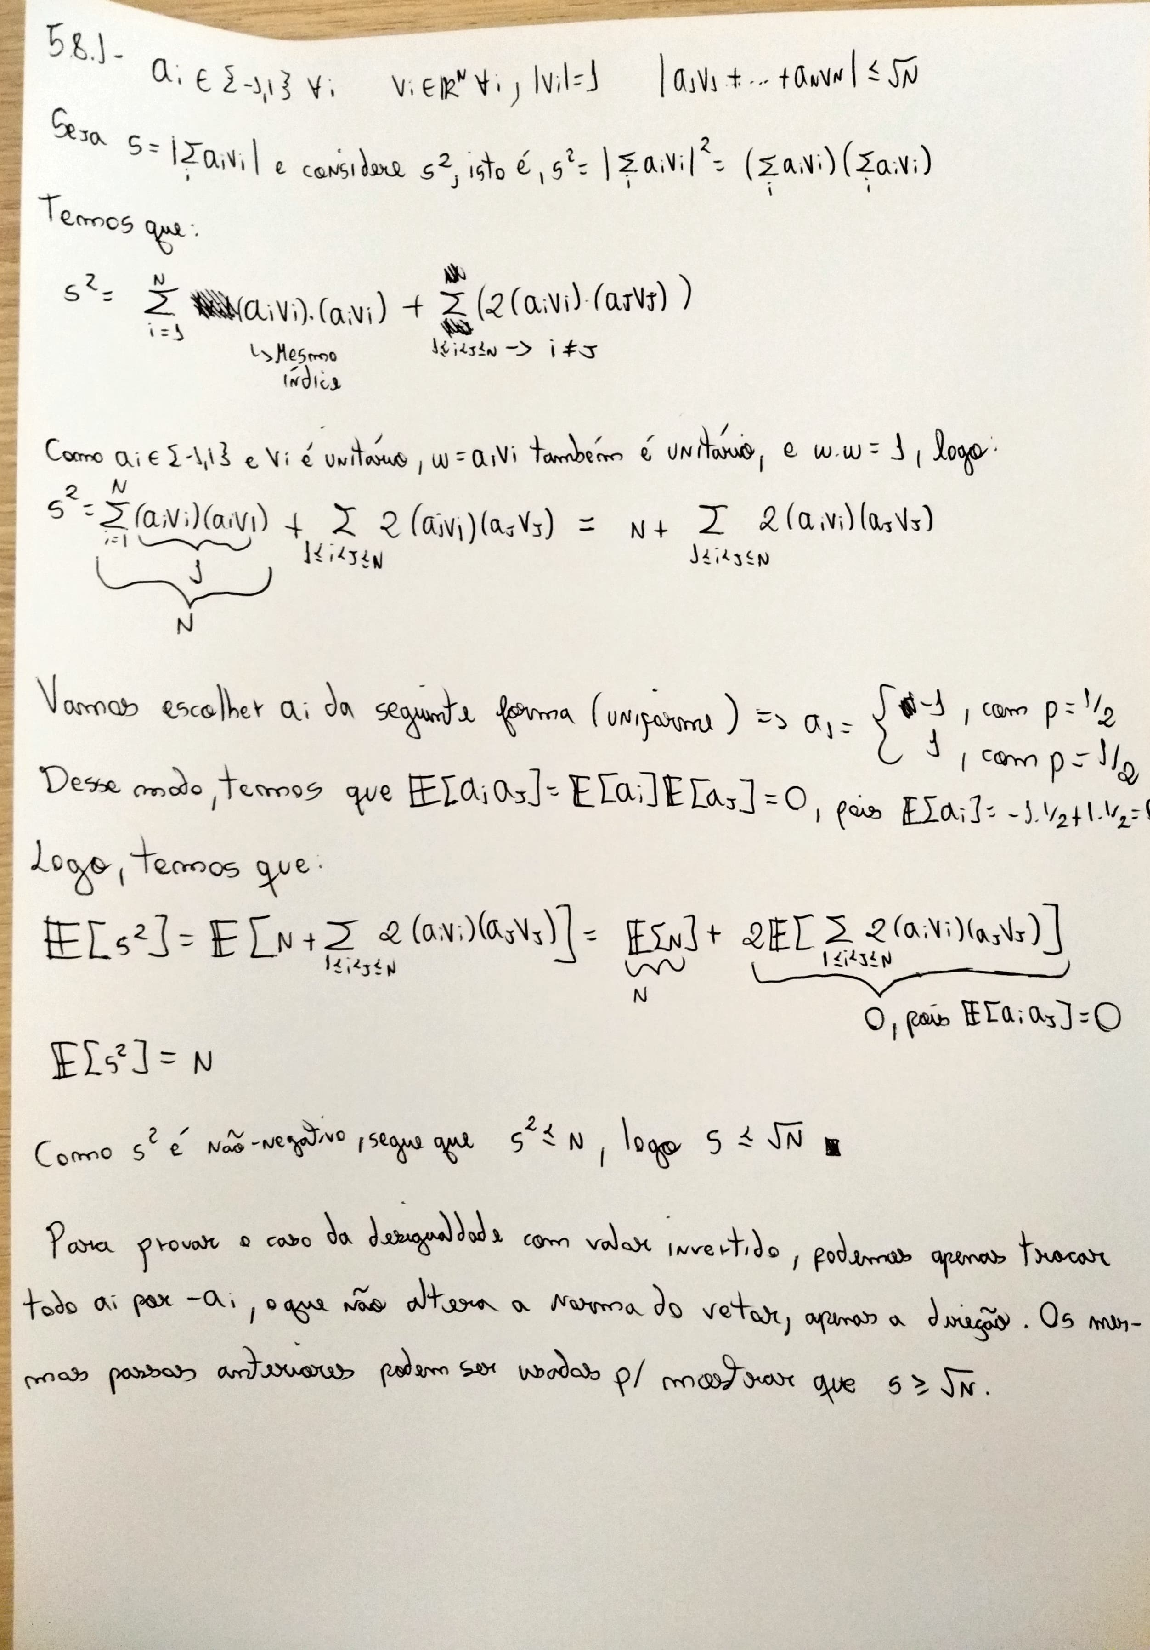
\includepdf[pages=-]{ex01.pdf}
\end{document}
